\chapter[Leif and His New Land]{
    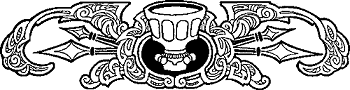
\includegraphics[width=9.3cm]{viking-tales/042}\\
    Leif and His New Land}

\lettrine{N}{ow} Eric had lived in Greenland for fifteen years. His sons
Thorstein and Leif had grown up to be big, strong men. One spring Leif
said to his father:

``I have never seen Norway, our mother land. I long to go there and meet
the great men and see the places that skalds sing about.''

Eric answered:

``It is right that you should go. No man has really lived until he has
seen Norway.''

So he helped Leif fit out a boat and sent him off. Leif sailed for
months. He passed Iceland and the Faroes and the Shetlands. He stopped
at all of these places and feasted his mind on the new things. And
everywhere men received him gladly; for he was handsome and wise. But at
last he came near Norway. Then he stood up before the pilot's seat and
sang loudly:

\begin{quote}
``My eyes can see her at last,\\
The mother of mighty men,\\
The field of famous fights.\\
In the sky above I see\\
Fair Asgard's shining roofs,\\
The flying hair of Thor,\\
The wings of Odin's birds,\\
The road that heroes tread.\\
I am here in the land of the gods,\\
The land of mighty men.''
\end{quote}

For a while he walked the land as though he were in a dream. He looked
at this and that and everything and loved them all because it was
Norway.

``I will go to the king,'' he said.

He had never seen a king. There were no kings in Iceland or in
Greenland. So he went to the city where the king had his fine house. The
king's name was Olaf. He was a great-grandson of Harald Hairfair; for
Harald had been dead a hundred years.

Now the king was going to hold a feast at night, and Leif put on his
most beautiful clothes to go to it. He put on long tights of blue wool
and a short jacket of blue velvet. He belted his jacket with a gold
girdle. He had shoes of scarlet with golden clasps. He threw around
himself a cape of scarlet velvet lined with seal fur. His long sword
stuck out from under his cloak. On his head he put a knitted cap of
bright colors. Then he walked to the king's feast hall and went through
the door. It was a great hall, and it was full of richly-dressed men.
The fires shone on so many golden head-bands and bracelets and so many
glittering swords and spears on the wall, and there was so much noise of
talking and laughing, that at first Leif did not know what to do. But at
last he went and sat on the very end seat of the bench near him.

As the feast went on, King Olaf sat in his high seat and looked about
the hall and noticed this one and that one and spoke across the fire to
many. He was keen-eyed and soon saw Leif in his far seat.

``Yonder is some man of mark,'' he said to himself. ``He is surely worth
knowing. His face is not the face of a fool. He carries his head like a
lord of men.''

He sent a thrall and asked Leif to come to him. So Leif walked down the
long hall and stood before the king.

``I am glad to have you for a guest,'' the king said. ``What are your
name and country?''

``I am Leif Ericsson, and I have come all the way from Greenland to see
you and old Norway.''

``From Greenland!'' said the king. ``It is not often that I see a
Greenlander. Many come to Norway to trade, but they seldom come to the
king's hall. I shall be glad to hear about your land. Come up and speak
with me.''

So Leif went up the steps of the high seat and sat down by the king and
talked with him. When the feast was over the king said:

``You shall live at my court this winter, Leif Ericsson. You are a
welcome guest.''

So Leif stayed there that winter. When he started back in the spring,
the king gave him two thralls as a parting gift.

``Let this gift show my love, Leif Ericsson,'' he said. ``For your sake
I shall not forget Greenland.''

Leif sailed back again and had good luck until he was past Iceland. Then
great winds came out of the north and tossed his ship about so that the
men could do nothing. They were blown south for days and days. They did
not know where they were. Then they saw land, and Leif said:

``Surely luck has brought us also to a new country. We will go in and
see what kind of a place it is.''

So he steered for it. As they came near, the men said:

``See the great trees and the soft, green shore. Surely this is a better
country than Greenland or than Iceland either.''

When they landed they threw themselves upon the ground.

``I never lay on a bed so soft as this grass,'' one said.

``Taller trees do not grow in Norway,'' said another.

``There is no stone here as in Norway, but only good black dirt,'' Leif
said. ``I never saw so fertile a land before.''

The men were hungry and set about building a fire.

``There is no lack of fuel here,'' they said.

They stayed many days in this country and walked about to see what was
there. A German, named Tyrker, was with Leif. He was a little man with a
high forehead and a short nose. His eyes were big and rolling. He had
lived with Eric for many years, and had taken care of Leif when he was a
little boy. So Leif loved him.

Now one day they had been wandering about and all came back to camp at
night except Tyrker. When Leif looked around on his comrades, he said:

``Where is Tyrker?''

No one knew. Then Leif was angry.

``Is a man of so little value in this empty land that you would lose
one?'' he said. ``Why did you not keep together? Did you not see that he
was gone? Why did you not set out to look for him? Who knows what
terrible thing may have happened to him in these great forests?''

Then he turned and started out to hunt for him. His men followed, silent
and ashamed. They had not gone far when they saw Tyrker running toward
them. He was laughing and talking to himself. Leif ran to him and put
his arms about him with gladness at seeing him.

\begin{figure}
    \centering
    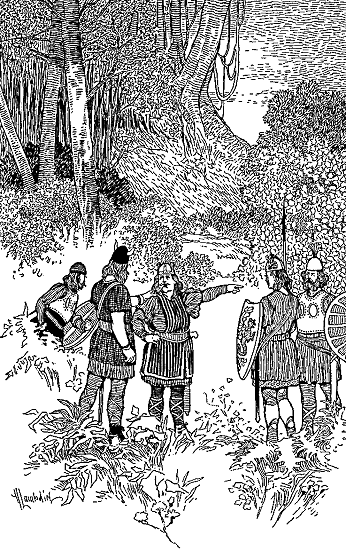
\includegraphics[width=9.1cm]{viking-tales/043}
    \caption{``He pointed to the woods and laughed and rolled his eyes''}
\end{figure}

``Why are you so late?'' he asked. ``Where have you been?''

But Tyrker, still smiling and nodding his head, answered in German. He
pointed to the woods and laughed and rolled his eyes. Again Leif asked
his question and put his hand on Tyrker's shoulder as though he would
shake him. Then Tyrker answered in the language of Iceland:

``I have not been so very far, but I have found something wonderful.''

``What is it?'' cried the men.

``I have found grapes growing wild,'' answered Tyrker, and he laughed,
and his eyes shone.

``It cannot be,'' Leif said.

Grapes do not grow in Greenland nor in Iceland nor even in Norway. So it
seemed a wonderful thing to these Norsemen.

``Can I not tell grapes when I see them?'' cried Tyrker. ``Did I not
grow up in Germany, where every hillside is covered with grapevines? Ah!
it seems like my old home.''

``It is wonderful,'' Leif said. ``I have heard travelers tell of seeing
grapes growing, but I myself never saw it. You shall take us to them
early in the morning, Tyrker.''

So in the morning they went back into the woods and saw the grapes. They
ate of them.

``They are like food and drink,'' they cried.

That day Leif said:

``We spent most of the summer on the ocean. Winter will soon be coming
on and the sea about Greenland will be frozen. We must start back. I
mean to take some of the things of this land to show to our people at
home. We will fill the rowboat with grapes and tow it behind us. The
ship we will load with logs from these great trees. That will be a
welcome shipload in Greenland, where we have neither trees nor vines.
Now half of you shall gather grapes for the next few days, and the other
half shall cut timber.''

So they did, and after a week sailed off. The ship was full of lumber,
and they towed the rowboat loaded with grapes. As they looked back at
the shore, Leif said:

``I will call this country Wineland for the grapes that grow there.''

One of the men leaped upon the gunwale and leaned out, clinging to the
sail, and sang:

\begin{quote}
``Wineland the good, Wineland the warm,\\
Wineland the green, the great, the fat.\\
Our dragon fed and crawls away\\
With belly stuffed and lazy feet.\\
How long her purple, trailing tail!\\
She fed and grew to twice her size.''
\end{quote}

Then all the men waved their hands to the shore and gave a great shout
for that good land.

For all that voyage they had fair weather and sailed into Eric's harbor
before the winter came. Eric saw the ship and ran down to the shore. He
took Leif into his arms and said:

``Oh, my son, my old eyes ached to see you. I hunger to hear of all that
you have seen and done.''

``Luck has followed me all the way,'' said Leif. ``See what I have
brought home.''

The Greenlanders looked.

``Lumber! lumber!'' they cried. ``Oh! it is better stuff than gold.''

Then they saw the grapes and tasted them.

``Surely you must have plundered Asgard,'' they said, smacking their
lips.

At the feast that night Eric said:

``Leif shall sit in the place of honor.''

So Leif sat in the high seat opposite Eric. All men thought him a
handsome and wise man. He told them of the storm and of Wineland.

``No man would ever need a cloak there. The soil is richer than the soil
of Norway. Grain grows wild, and you yourselves saw the grapes that we
got from there. The forests are without end. The sea is full of fish.''

The Greenlanders listened with open mouths to all this. They turned and
talked to Leif's ship-comrades who were scattered among them.

Leif noticed two strangers, an old man who sat at Eric's side and a
young woman on the cross-bench. He turned to his brother Thorstein who
sat next to him.

``Who are these strangers?'' he asked.

``Thorbiorn and his daughter Gudrid,'' Thorstein answered. ``They landed
here this spring. I never saw our father more glad of anything than to
see this Thorbiorn. They were friends before we left Iceland. When they
saw each other again they could not talk enough of old times. In the
spring Eric means to give him a farm up the fiord a way. It seems that
this Thorbiorn comes of a good family that has been rich and great in
Iceland for years. And Thorbiorn himself was rich when our father knew
him, and was much honored by all men. But ill luck came, and he grew
poor. This hurt his pride. `I will not stay in Iceland and be a beggar,'
he said to himself. `I will not have men look at me and say, ``He is not
what his father was.'' I will go to my friend Eric the Red in
Greenland.'

``Then he got ready a great feast and invited all his friends. It was
such a feast as had not been in Iceland for years. Thorbiorn spent on it
all the wealth that he had left. For he said to himself, `I will not
leave in shame. Men shall remember my last feast.' After that he set out
and came to Greenland.

``Is not Gudrid beautiful? And she is wise. I mean to marry her, if her
father will permit it.''

Now Leif settled down in Greenland and became a great man there. He was
so busy and he grew so rich that he did not think of going to Wineland
again. But people could not forget his story. Many nights as men sat
about the long fires they talked of that wonderful land and wished to
see it.

\begin{figure}[hb]
    \centering
    \vskip8pt
    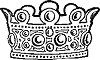
\includegraphics[width=2.7cm]{viking-tales/014}
\end{figure}
